\documentclass[a4paper,anonymous,USenglish]{lipics-v2019}
%\nolinenumbers\hideLIPIcs
\usepackage[utf8]{inputenc}
\usepackage{algorithm}
\usepackage{algpseudocode} % for pseudocode
\usepackage{tikz} % for figures
\usepackage{subcaption} % for subfigures

\hyphenation{time-stamp time-stamps re-con-cilia-tion}
\renewcommand{\floatpagefraction}{.8}%

\title{Byzantine Eventual Consistency and Byzantine Causal Broadcast}

\author{Martin Kleppmann}{University of Cambridge}{mk428@cst.cam.ac.uk}{https://orcid.org/0000-0001-7252-6958}{Supported by a Leverhulme Trust Early Career Fellowship and by the Isaac Newton Trust.}

\author{Heidi Howard}{University of Cambridge}{hh360@cst.cam.ac.uk}{https://orcid.org/0000-0001-5256-7664}{}

\authorrunning{M. Kleppmann and H. Howard}
\Copyright{Martin Kleppmann and Heidi Howard}

\begin{CCSXML}
<ccs2012>
  <concept>
    <concept_id>10003752.10003809.10010172</concept_id>
    <concept_desc>Theory of computation~Distributed algorithms</concept_desc>
    <concept_significance>500</concept_significance>
  </concept>
  <concept>
    <concept_id>10002951.10003152.10003166.10003172</concept_id>
    <concept_desc>Information systems~Remote replication</concept_desc>
    <concept_significance>300</concept_significance>
  </concept>
  <concept>
    <concept_id>10010520.10010575</concept_id>
    <concept_desc>Computer systems organization~Dependable and fault-tolerant systems and networks</concept_desc>
    <concept_significance>300</concept_significance>
  </concept>
  <concept>
    <concept_id>10002978.10003014.10003015</concept_id>
    <concept_desc>Security and privacy~Security protocols</concept_desc>
    <concept_significance>300</concept_significance>
  </concept>
</ccs2012>
\end{CCSXML}

\ccsdesc[500]{Theory of computation~Distributed algorithms}
\ccsdesc[300]{Information systems~Remote replication}
\ccsdesc[300]{Computer systems organization~Dependable and fault-tolerant systems and networks}
\ccsdesc[300]{Security and privacy~Security protocols}

\keywords{replication, Byzantine fault tolerance, eventual consistency, CRDTs, broadcast protocols}

\begin{document}
\maketitle
\begin{abstract}
    Byzantine agreement algorithms guarantee consistency and liveness on the condition that a bounded number of processes (typically $1/3$) are faulty; they provide no guarantees if that bound is exceeded.
    However, if more faults occur, we can still guarantee weaker consistency models. 
    In this paper we define one such model, which we call \emph{Byzantine Eventual Consistency} (BEC).
    It builds upon a \emph{Byzantine Causal Broadcast} protocol; we introduce algorithms that implement this protocol, even in a system with arbitrarily many Byzantine-faulty processes, and we prove their correctness.
    We show that the performance of our final algorithm is near optimal in terms of network bandwidth and round-trips.
\end{abstract}
\maketitle\\[20pt]
This paper is not eligible for the best student paper award.
\newpage

\section{Introduction}

Byzantine agreement assumes that at most $f$ out of $n$ processes are Byzantine-faulty.
It is well established that without synchrony, Byzantine agreement is impossible if $n\leq3f$~\cite{Dwork:1988,Lamport:1982}.
If more than $f$ processes are faulty, neither safety (agreement) nor liveness can be guaranteed.

In practice, the assumption that no more than $f$ processes are faulty is not always a realistic threat model.
Byzantine failures are not necessarily independent: if an adversary can compromise one of the processes (e.g. due to a software vulnerability), it is likely that they can compromise a majority of processes, since they are probably all running the same software. 
Similarly, non-malicious software bugs are likely to affect many of the processes at once.
This issue was acknowledged in the pBFT paper~\cite{Castro:1999}, which states that: ``{\dots}each node should run different implementations of the service code and operating system{\dots}''~--- an assumption that is unrealistic for any system with more than a few processes, and is seldom true in practice today.
Moreover, in some systems, such as open peer-to-peer networks that anybody can join, an adversary can spawn a large number of processes, and thus create a majority of Byzantine-faulty processes (this is known as a Sybil attack~\cite{Douceur:2002}).
In such systems it is not appropriate to assume a bound on the number of Byzantine-faulty processes.

This state of affairs raises the question: if Byzantine agreement cannot be achieved in the face of arbitrary numbers of Byzantine-faulty processes, is there a consistency model we \emph{can} achieve under this assumption?

To answer this question, this paper first introduces two algorithms for \emph{Byzantine causal broadcast} (\S~\ref{sec:algorithm}), a mechanism for broadcasting (multicasting) messages to a group of processes (defined in \S~\ref{sec:background}).
Unlike previous approaches, e.g.\ using vector clocks, our algorithms provide casual broadcast in the presence of any number of Byzantine-faulty processes.
We prove the correctness of our algorithms (Appendix~\ref{sec:proof}) and demonstrate experimentally that our second algorithm has near-optimal network communication cost (\S~\ref{sec:evaluation}).

We then combine Byzantine causal broadcast with existing work on \emph{Conflict-free Replicated Data Types} (CRDTs) to implement Byzantine fault-tolerant replicated storage  (\S~\ref{sec:byzantine-crdts}).
For this storage we propose \emph{Byzantine Eventual Consistency} (BEC), a novel consistency model that can be achieved in systems with arbitrarily many Byzantine-faulty processes.
BEC ensures that all correct replicas converge towards the same shared state, even if they also communicate with any number of Byzantine-faulty processes.
Essentially, BEC ensures that faulty replicas cannot permanently corrupt the state of correct replicas.

\section{Background}\label{sec:background}

Algorithms for Byzantine agreement (or consensus) are often used to create an append-only log of values such as a blockchain~\cite{Bano:2019}, or, equivalently, a \emph{total order broadcast} protocol~\cite{Cachin:2011wt,Defago:2004ji}.
A total order broadcast (a.k.a.\ \emph{atomic broadcast}) protocol allows messages to be sent to a group of processes.
It is defined in terms of two primitives, \emph{broadcast} and \emph{deliver}, and must satisfy the following properties:

\begin{description}
\item[Validity:] If a correct process delivers a message $m$ with sender $s$, then $m$ was broadcast by $s$.
\item[Non-duplication:] A correct process does not deliver the same message more than once.
\item[Self-delivery:] If a correct process $p$ broadcasts a message $m$, then $p$ eventually delivers $m$.
\item[Eventual delivery:] If a correct process delivers a message $m$, then all correct processes will eventually deliver $m$.
\item[Total order:] If a correct process delivers message $m_1$ before delivering message $m_2$, then all correct processes must deliver $m_1$ before $m_2$.
\end{description}

Byzantine agreement algorithms can ensure these properties assuming that no more than $f$ out of $n$ processes are faulty (see \S~\ref{sec:relwork}).
To ensure eventual delivery we must also assume partial synchrony~\cite{Dwork:1988}.
The \emph{state machine replication} approach~\cite{Schneider:1990} can be used to implement strongly consistent (linearizable) replicated storage on top of total order broadcast.
%State machine replication treats every replica as a deterministic state machine, where the inputs are commands.
%If all replicas observe the same commands in the same order, they all go through the same sequence of state transitions, resulting in the same final state.

\emph{Causal broadcast}~\cite{Birman:1991el,Cachin:2011wt} is also defined by five properties, of which the first four are identical to total order broadcast.
The total order property is replaced with a weaker one:

\begin{description}
\item[Causal order:] If a correct process broadcasts or delivers $m_1$ before broadcasting message $m_2$, then all correct processes must deliver $m_1$ before delivering $m_2$.
\end{description}

This imposes a partial order on messages: $m_1$ must be delivered before $m_2$ if $m_2$ has a causal dependency on $m_1$, but concurrently sent messages can be delivered in any order.

\begin{figure}
\centering
\begin{minipage}{.5\textwidth}
    \centering
    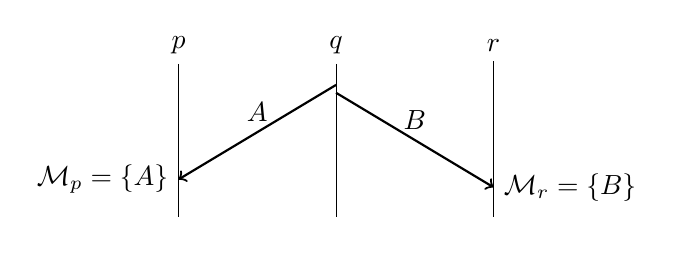
\begin{tikzpicture}
% Timelimes
\node (p-start) at (0, 0.5) {$p$};
\node (p-end)   at (0, -1.8) {};
\node (q-start) at (2, 0.5) {$q$};
\node (q-end)   at (2, -1.8) {};
\node (r-start) at (4, 0.5) {$r$};
\node (r-end)   at (4, -1.8) {};
\draw (p-start) -- (p-end);
\draw (q-start) -- (q-end);
\draw (r-start) -- (r-end);

% Messages
\draw[thick,->] (2, 0) to node [above] {$A$} (0, -1.2) node [left] {$\mathcal{M}_p = \{A\}$};

\draw[thick,->] (2, -0.1) to node [above] {$B$} (4, -1.3) node [right] {$\mathcal{M}_r = \{B\}$};

\end{tikzpicture}

    \captionsetup{width=.95\linewidth}
    \caption{Byzantine-faulty process $q$ sends conflicting messages to correct processes $p$ and $r$.
    The sets $\mathcal{M}_p$ and ${M}_r$ do not converge.}
    \label{fig:trivial1}
\end{minipage}%
\begin{minipage}{.5\textwidth}
    \centering
    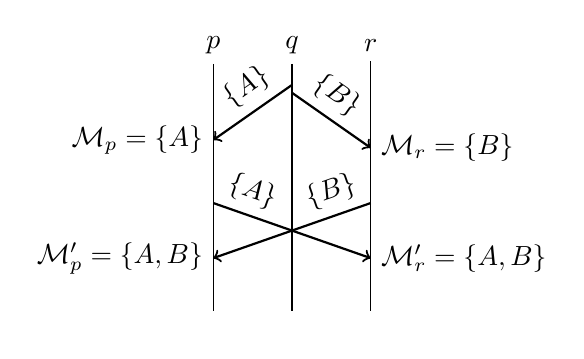
\begin{tikzpicture}

% Space between timelines
\def\width{1}
% Message delay
\def\delay{0.7}

% Timelimes
\node (p-start) at (0, 0.5) {$p$};
\node (p-end)   at (0, -3) {};
\node (q-start) at (\width, 0.5) {$q$};
\node (q-end)   at (\width, -3) {};
\node (r-start) at (\width*2, 0.5) {$r$};
\node (r-end)   at (\width*2, -3) {};
\draw (p-start) -- (p-end);
\draw (q-start) -- (q-end);
\draw (r-start) -- (r-end);

% Messages
\draw[thick,->] (\width, 0) to node [above,pos=0.4,sloped] {$\{A\}$} (0, -\delay) node [left] {$\mathcal{M}_p = \{A\}$};

\draw[thick,->] (\width, -0.1) to node [above,pos=0.4,sloped] {$\{B\}$} (\width*2, -\delay-0.1) node [right] {$\mathcal{M}_r = \{B\}$};

\draw[thick,->] (0, -1.5) to node [above,pos=0.2,sloped] {$\{A\}$} (\width*2, -1.5-\delay) node [right] {$\mathcal{M}_r' = \{A,B\}$};

\draw[thick,->] (\width*2, -1.5) to node [above,pos=0.2,sloped] {$\{B\}$} (0, -1.5-\delay) node [left] {$\mathcal{M}_p' = \{A,B\}$};

\end{tikzpicture}

% \begin{tikzpicture}
% % Timelimes
% \node (p-start) at (0, 0.5) {$p$};
% \node (p-end)   at (0, -3.4) {};
% \node (q-start) at (2, 0.5) {$q$};
% \node (q-end)   at (2, -3.4) {};
% \node (r-start) at (4, 0.5) {$r$};
% \node (r-end)   at (4, -3.4) {};
% \draw (p-start) -- (p-end);
% \draw (q-start) -- (q-end);
% \draw (r-start) -- (r-end);

% % Messages
% \draw[thick,->] (2, 0) to node [above] {$\{A\}$} (0, -1.2) node [left] {$\mathcal{M}_p = \{A\}$};

% \draw[thick,->] (2, -0.1) to node [above] {$\{B\}$} (4, -1.3) node [right] {$\mathcal{M}_r = \{B\}$};

% \draw[thick,->] (0, -1.7) to node [above,pos=0.25] {$\{A\}$} (4, -2.9) node [right] {$\mathcal{M}_r' = \{A,B\}$};

% \draw[thick,->] (4, -1.7) to node [above,pos=0.25] {$\{B\}$} (0, -2.9) node [left] {$\mathcal{M}_p' = \{A,B\}$};

% \end{tikzpicture}

    \captionsetup{width=.95\linewidth}
    \caption{As correct processes $p$ and $r$ reconcile their sets of messages, they converge to the same set $\mathcal{M}_p' = \mathcal{M}_r' = \{A,B\}$.}
    \label{fig:trivial2}
\end{minipage}
\end{figure}

\subsection{Na\"{\i}ve broadcast algorithms}

The simplest broadcast algorithm is as follows: every time a process wants to broadcast a message, it delivers that message to itself, and also sends that message to each other process via a pairwise link, re-transmitting until it is acknowledged.
However, this algorithm does not provide the \emph{eventual delivery} property in the face of Byzantine-faulty processes, as shown in Figure~\ref{fig:trivial1}: a faulty process $q$ may send two different messages $A$ and $B$ to correct processes $p$ and $r$, respectively; then $p$ never delivers $B$ and $r$ never delivers $A$.

To address this issue, processes $p$ and $r$ must communicate with each other (either directly, or indirectly via other correct processes).
Let $\mathcal{M}_p$ and $\mathcal{M}_r$ be the set of messages delivered by processes $p$ and $r$, respectively.
Then, as shown in Figure~\ref{fig:trivial2}, $p$ can send its entire set $\mathcal{M}_p$ to $r$, and $r$ can send $\mathcal{M}_r$ to $p$, so that both processes can compute $\mathcal{M}_p \cup \mathcal{M}_r$, and deliver any new messages.
Pairs of processes can thus periodically \emph{reconcile} their sets of delivered messages.

Adding this reconciliation process to the broadcast protocol ensures the first four properties of causal broadcast.
Additional mechanisms are required to ensure the fifth property, \emph{casual order}.
However, this algorithm is very inefficient: when processes periodically reconcile their state, we can expect that at the start of each round of reconciliation their sets of messages already have many elements in common.
Sending the entire set of messages to each other thus implies transmitting a large amount of data unnecessarily.

An efficient reconciliation algorithm should determine which messages have already been delivered by both processes, and transmit only those messages that are unknown to the other process.
For example, process $p$ should only send $\mathcal{M}_p \setminus \mathcal{M}_r$ to process $r$, and process $r$ should only send $\mathcal{M}_r \setminus \mathcal{M}_p$ to process $p$.
The algorithm should also complete in a small number of round-trips and minimise the size of messages sent.
These goals rule out other na\"{\i}ve approaches too: for example, instead of sending all messages in $\mathcal{M}_p$, process $p$ could send the hash of each message in $\mathcal{M}_p$, which can be used by other processes to determine which messages they are missing; this is still inefficient, as the message size is $O(|\mathcal{M}_{p}|)$.

\begin{figure}
    \centering
    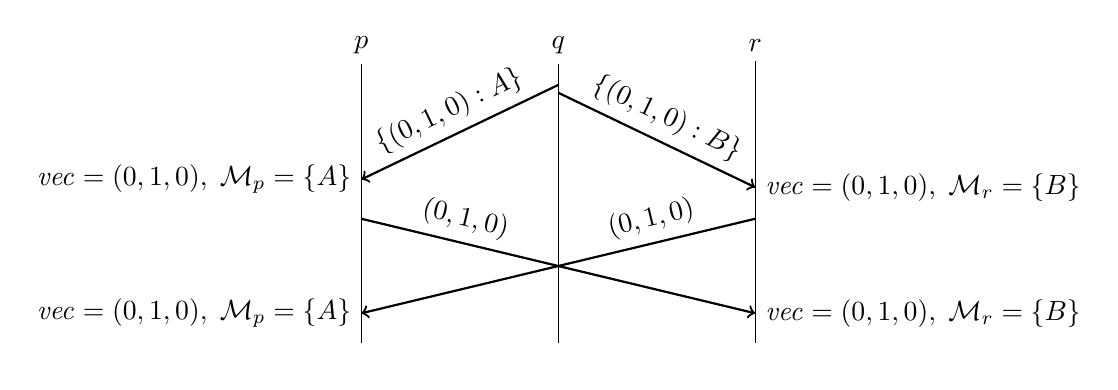
\begin{tikzpicture}
% Timelimes
\node (p-start) at (0, 0.5) {$p$};
\node (p-end)   at (0, -3.4) {};
\node (q-start) at (2.5, 0.5) {$q$};
\node (q-end)   at (2.5, -3.4) {};
\node (r-start) at (5, 0.5) {$r$};
\node (r-end)   at (5, -3.4) {};
\draw (p-start) -- (p-end);
\draw (q-start) -- (q-end);
\draw (r-start) -- (r-end);

% Messages
\draw[thick,->] (2.5, 0) to node [above,sloped] {$\{(0,1,0): A\}$} (0, -1.2) node [left] {$\mathit{vec} = (0,1,0),\; \mathcal{M}_p = \{A\}$};

\draw[thick,->] (2.5, -0.1) to node [above,sloped] {$\{(0,1,0): B\}$} (5, -1.3) node [right] {$\mathit{vec} = (0,1,0),\; \mathcal{M}_r = \{B\}$};

\draw[thick,->] (0, -1.7) to node [above,pos=0.25,sloped] {$(0,1,0)$} (5, -2.9) node [right] {$\mathit{vec} = (0,1,0),\; \mathcal{M}_r = \{B\}$};

\draw[thick,->] (5, -1.7) to node [above,pos=0.25,sloped] {$(0,1,0)$} (0, -2.9) node [left] {$\mathit{vec} = (0,1,0),\; \mathcal{M}_p = \{A\}$};

\end{tikzpicture}

    \caption{Processes $p$ and $r$ believe they are in the same state because their vector timestamps are the same, when in fact their sets of messages are inconsistent due to $q$'s faulty behaviour.}
    \label{fig:vectorclocks}
\end{figure}

\subsection{Vector clocks}

Non-Byzantine causal broadcast algorithms often rely on \emph{vector clocks} to determine which messages to send to each other, and how to order them~\cite{Birman:1991el,Schwarz:1994}.
However, vector clocks are not suitable in a Byzantine setting.
The problem is illustrated in Figure~\ref{fig:vectorclocks}, where faulty process $q$ generates two different messages, $A$ and $B$, with the same vector timestamp $(0, 1, 0)$.

In a system where processes correctly follow the protocol, the three components of the timestamp represent the number of distinct messages broadcast by $p$, $q$, and $r$ respectively.
Thus, $p$ and $r$ should be able to reconcile their sets of messages by first sending each other their latest vector timestamps, which serve as a concise summary of the set of messages they have seen.
However, in the example of Figure~\ref{fig:vectorclocks}, this approach fails due to $q$'s earlier faulty behaviour: $p$ and $r$ detect that their vector timestamps are equal, and thus incorrectly believe that they are in the same state, even though their sets of messages are different.

Thus, vector clocks can be corrupted by a faulty process; a Byzantine-fault-tolerant causal broadcast algorithm must not be vulnerable to such corruption.

\subsection{System Model}\label{sec:system-model}

Our system consists of any number of processes, each of which is either \emph{correct} or \emph{faulty}, but one process does not know whether another process is faulty.
A correct process follows the specified protocol, whereas a faulty process may deviate from the protocol in arbitrary ways (i.e.\ it is Byzantine-faulty).
We model this by assuming a malicious adversary who controls the behaviour of all faulty processes.
We allow any number of processes to be faulty.
We treat all processes as equal, making no distinction e.g.\ between clients and servers.

We assume that each process has a distinct private key that can be used for digital signatures, and that the corresponding public key is known to all processes.
We assume that no process knows the private key of another process, and thus signatures cannot be forged.

Processes communicate by sending messages over pairwise network links.
Not all pairs of processes are necessarily connected with a network link.
We assume that all messages sent over these links are signed by the sender, and the recipient ignores messages with invalid signatures.
Thus, even if the adversary can tamper with network traffic, it can only cause message loss but not impersonate a correct process.
We model message loss using fair-loss links~\cite{Cachin:2011wt}: that is, if processes repeatedly retransmit a message, it will eventually be received.

We assume an asynchronous system with unbounded message delay and arbitrary differences in speed of different processes.
For the sake of eventual delivery, we must assume that in the graph of processes and network links, the correct processes form a single connected component.
This assumption is necessary because if there are two correct processes that can only ever communicate via faulty processes, then no algorithm can guarantee eventual delivery, because the adversary can always block communication between the correct processes.

% State the assumption of a collision-free hash function as part of the system model?

% As is standard in Byzantine systems, we can only reason about the behaviour of correct processes, since we make no assumptions about the behaviour or internal state of faulty processes.


\section{Byzantine Causal Broadcast}\label{sec:algorithm}

We now present two causal broadcast algorithms that tolerate any number of Byzantine-faulty processes.
At their core is a reconciliation algorithm that ensures two processes have delivered the same set of broadcast messages, in causal order.
The reconciliation is efficient in the sense that when two correct processes communicate, they only exchange broadcast messages that the other process has not already delivered.

\subsection{A hash graph of messages}

Let $\mathcal{M}$ be the set of broadcast messages delivered by the current process.
$\mathcal{M}$ is a set of triples $(v, \mathit{hs}, \mathit{sig})$, where $v$ is any value, $\mathit{sig}$ is a digital signature over $(v, \mathit{hs})$ using the sender's private key, and $\mathit{hs}$ is a set of hashes produced by a cryptographic hash function $H(\cdot)$, such as SHA-256.
We assume that $H$ is collision-resistant, i.e.\ that it is computationally infeasible to find distinct $x$ and $y$ such that $H(x) = H(y)$.

Let $A, B \in \mathcal{M}$, where $B = (v, \mathit{hs}, \mathit{sig})$ and $H(A) \in \mathit{hs}$.
Then we call $A$ a \emph{predecessor} of $B$, and $B$ a \emph{successor} of $A$.
Define a graph with a vertex for each message in $\mathcal{M}$, and a directed edge from each message to each of its predecessors.
We can assume that this graph is acyclic because the presence of a cycle would imply knowledge of a collision in the hash function.
Figure~\ref{fig:example-dags} shows examples of such graphs.

Let $\mathrm{succ}^1(\mathcal{M}, m)$ be the set of successors of message $m$ in $\mathcal{M}$, let $\mathrm{succ}^2(\mathcal{M}, m)$ be the successors of the successors of $m$, and so on, and let $\mathrm{succ}^*(\mathcal{M}, m)$ be the transitive closure:
\begin{align*}
\mathrm{succ}^i(\mathcal{M}, m) &=
\begin{cases}
\{(v, \mathit{hs}, \mathit{sig}) \in \mathcal{M} \mid H(m) \in \mathit{hs}\} & \text{ for } i=1 \\
\bigcup_{m' \in \mathrm{succ}^1(\mathcal{M}, m)} \mathrm{succ}^{i-1}(\mathcal{M}, m') & \text{ for } i>1
\end{cases} \\
\mathrm{succ}^*(\mathcal{M}, m) &= \bigcup_{i \ge 1} \mathrm{succ}^i(\mathcal{M}, m)
\end{align*}
We define the set of predecessors of $m$ similarly:
\begin{align*}
\mathrm{pred}^i(\mathcal{M}, m) &=
\begin{cases}
\{ m' \in \mathcal{M} \mid m = (v, \mathit{hs}, \mathit{sig}) \wedge H(m') \in \mathit{hs}\} & \text{ for } i=1 \\
\bigcup_{m' \in \mathrm{pred}^1(\mathcal{M}, m)} \mathrm{pred}^{i-1}(\mathcal{M}, m') & \text{ for } i>1
\end{cases} \\
\mathrm{pred}^*(\mathcal{M}, m) &= \bigcup_{i \ge 1} \mathrm{pred}^i(\mathcal{M}, m)
\end{align*}
Let $\mathrm{heads}(\mathcal{M})$ denote the set of hashes of those messages in $\mathcal{M}$ that have no successors:
\[ \mathrm{heads}(\mathcal{M}) = \{H(m) \mid m \in \mathcal{M} \wedge \mathrm{succ}^1(\mathcal{M}, m) = \{\}\;\}. \]

\subsection{A first Byzantine fault-tolerant reconciliation algorithm}\label{sec:algorithm1}

We assume that communication between two processes takes place over a \emph{connection}.
This connection is a logical grouping of a bidirectional sequence of related request/response messages between two processes (in practice, it can be implemented as a TCP connection).
Connections have the same fair-loss assumption as individual message delivery: messages may be dropped, resulting in the connection eventually timing out, and the reconciliation process being cancelled.
However, if two processes repeatedly try, eventually they will succeed in creating a connection of finite duration that is free from message loss.

When a correct process wishes to broadcast a message with value $v$, it executes lines~\ref{line:broadcast-begin}--\ref{line:broadcast-end} of Algorithm~\ref{fig:algorithm}: it constructs a message $m$ containing the current heads and a signature, sends $m$ via all connections, delivers $m$ to itself, and adds $m$ to the set of locally delivered messages $\mathcal{M}$.
However, this is not sufficient to ensure eventual delivery, since some processes may be disconnected, and faulty nodes might not correctly follow this protocol.

To ensure eventual delivery, we assume that processes periodically attempt to reconnect to each other.
When such a connection is established, the processes reconcile their sets of messages to discover any missing messages.
If two processes are not able to connect directly, they can still exchange messages by periodically reconciling with one or more correct intermediary processes (as stated in \S~\ref{sec:system-model}, we assume that such intermediaries exist).

\algblockdefx{On}{EndOn}[1]{\textbf{on} #1 \textbf{do}}{\textbf{end on}}
\begin{algorithm}
    \begin{algorithmic}[1]
    \On{request to broadcast $v$}\label{line:broadcast-begin}
        \State $\mathit{hs} := \mathrm{heads}(\mathcal{M})$\label{line:broadcast-heads}
        \State $\mathit{sig} := \text{signature over } (v, \mathit{hs}) \text{ using this process's private key}$
        \State $m := (v, \mathit{hs}, \mathit{sig})$
        \State \textbf{send} $\langle\mathsf{msgs}: \{m\}\rangle$ via all active connections\label{line:eager-send}
        \State \textbf{deliver} $m$ to self
        \State $\mathcal{M} := \mathcal{M} \cup \{m\}$
    \EndOn\label{line:broadcast-end}
    \State
    \On{connecting to another process} \label{line:connect-begin}
        \State $\mathit{sent} := \{\};\; \mathit{recvd} := \{\};\; \mathit{missing} := \{\};\; \mathcal{M}_\mathsf{conn} := \mathcal{M}$ \label{line:init}\Comment{connection-local variables}
        \State \textbf{send} $\langle\mathsf{heads}: \mathrm{heads}(\mathcal{M}_\mathsf{conn})\rangle$ via current connection \label{line:send-heads}
    \EndOn \label{line:connect-end}
    \State
    \On{receiving $\langle\mathsf{heads}: \mathit{hs}\rangle$ via a connection} \label{line:recv-heads}
        \State \Call{HandleMissing}{$\{h \in \mathit{hs} \mid \nexists m \in \mathcal{M}_\mathsf{conn}.\; H(m) = h\}$} \label{line:heads-missing}
    \EndOn\label{line:recv-heads-end}
    \State
    \On{receiving $\langle\mathsf{msgs}: \mathit{new}\rangle$ via a connection} \label{line:recv-msgs}
        \State $\mathit{recvd} := \mathit{recvd} \,\cup\, \{(v, \mathit{hs}, \mathit{sig}) \in \mathit{new} \mid \mathit{sig}\text{ is a valid process' signature over }(v, \mathit{hs}) \}$ \label{line:msgs-recvd}
        \State $\mathit{unresolved} := \{h \mid \exists (v, \mathit{hs}, \mathit{sig}) \in \mathit{recvd}.\; h \in \mathit{hs} \;\wedge\; \nexists m \in (\mathcal{M}_\mathsf{conn} \cup \mathit{recvd}).\; H(m) = h\}$ \label{line:msgs-missing}
        \State \Call{HandleMissing}{$\mathit{unresolved}$} \label{line:msgs-handle-missing}
    \EndOn\label{line:recv-msgs-end}
    \State
    \On{receiving $\langle\mathsf{needs}: \mathit{hashes}\rangle$ via a connection} \label{line:recv-needs}
        \State $\mathit{reply} := \{m \in \mathcal{M}_\mathsf{conn} \mid H(m) \in \mathit{hashes} \,\wedge\, m \notin \mathit{sent}\}$ \label{line:needs-reply}
        \State $\mathit{sent} := \mathit{sent} \cup \mathit{reply}$
        \State \textbf{send} $\langle\mathsf{msgs}: \mathit{reply}\rangle$ via current connection \label{line:send-msgs}
    \EndOn\label{line:end-needs}
    \State
    \Function{HandleMissing}{$\mathit{hashes}$}
        \State $\mathit{missing} := (\mathit{missing} \cup \mathit{hashes}) \setminus \{H(m) \mid m \in \mathit{recvd}\}$
        \If{$\mathit{missing} = \{\}$} \label{line:missing-empty}
            \State \textbf{deliver} all of the messages in $\mathit{recvd} \setminus \mathcal{M}$ in topologically sorted order\label{line:deliver}
            \State $\mathcal{M} := \mathcal{M} \cup \mathit{recvd}$ \label{line:update-m}
            \State optionally \textbf{send} $\langle\mathsf{msgs}: \mathit{recvd} \setminus \mathcal{M}\rangle$ via all other connections\label{line:eager-relay}
            \State \textbf{reconciliation complete} \label{line:finish}
        \Else
            \State \textbf{send} $\langle\mathsf{needs}: \mathit{missing}\rangle$ via current connection \label{line:send-missing}
        \EndIf
    \EndFunction
    \end{algorithmic}
    \caption{A Byzantine fault tolerant causal broadcast algorithm.}\label{fig:algorithm}
\end{algorithm}

% hspace is an ugly hack to get the figure to line up as dag-after has some extra whitespace
\begin{figure}
    \centering
    \begin{subfigure}[b]{0.35\textwidth}
    \centering
    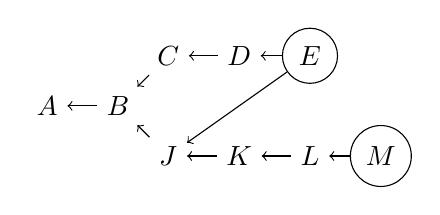
\begin{tikzpicture}[node distance=0.9cm]

% nodes
\node (a) {$A$};
\node (b) [right of=a] {$B$};
\node (c) [above right of=b] {$C$};
\node (d) [right of=c] {$D$};
\node (e) [right of=d,draw,circle] {$E$};
\node (j) [below right of=b] {$J$};
\node (k) [right of=j] {$K$};
\node (l) [right of=k] {$L$};
\node (m) [right of=l,draw,circle] {$M$};

% arrows
\draw[<-] (a) -- (b);
\draw[<-] (b) -- (c);
\draw[<-] (c) -- (d);
\draw[<-] (d) -- (e);
\draw[<-] (j) -- (e);
\draw[<-] (b) -- (j);
\draw[<-] (j) -- (k);
\draw[<-] (k) -- (l);
\draw[<-] (l) -- (m);
\end{tikzpicture}\hspace{0.5cm}
    \captionsetup{width=.9\linewidth}
    \caption{Messages at $p$ before reconciliation.}
    \end{subfigure}%
    \begin{subfigure}[b]{0.26\textwidth}
    \centering
    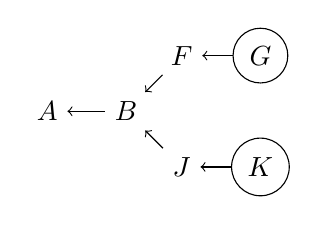
\begin{tikzpicture}

% nodes
\node (a) {$A$};
\node (b) [right of=a] {$B$};
\node (f) [above right of=b] {$F$};
\node (g) [right of=f,circle,draw] {$G$};
\node (j) [below right of=b] {$J$};
\node (k) [right of=j,circle,draw] {$K$};

% arrows
\draw[<-] (a) -- (b);
\draw[<-] (b) -- (f);
\draw[<-] (f) -- (g);
\draw[<-] (b) -- (j);
\draw[<-] (j) -- (k);
\end{tikzpicture}\hspace{0.5cm}
    \captionsetup{width=.9\linewidth}
    \caption{Messages at $q$ before reconciliation.}
    \end{subfigure}%
    \begin{subfigure}[b]{0.35\textwidth}
    \centering
    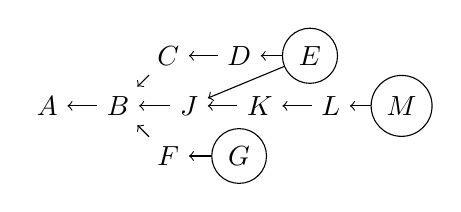
\begin{tikzpicture}[node distance=0.9cm]

% nodes
\node (a) {$A$};
\node (b) [right of=a] {$B$};
\node (c) [above right of=b] {$C$};
\node (d) [right of=c] {$D$};
\node (e) [right of=d,draw,circle] {$E$};
\node (j) [right of=b] {$J$};
\node (k) [right of=j] {$K$};
\node (l) [right of=k] {$L$};
\node (m) [right of=l,draw,circle] {$M$};
\node (f) [below right of=b] {$F$};
\node (g) [right of=f,draw,circle] {$G$};

% arrows
\draw[<-] (a) -- (b);
\draw[<-] (b) -- (c);
\draw[<-] (c) -- (d);
\draw[<-] (d) -- (e);
\draw[<-] (b) -- (j);
\draw[<-] (j) -- (e);
\draw[<-] (j) -- (k);
\draw[<-] (k) -- (l);
\draw[<-] (l) -- (m);
\draw[<-] (b) -- (f);
\draw[<-] (f) -- (g);
\end{tikzpicture}
    \captionsetup{width=.9\linewidth}
    \caption{Messages at $p$ and $q$ after reconciliation.}
    \end{subfigure}
    \caption{Example DAGs of delivered messages. Arrows represent a message referencing the hash of its predecessor, and heads (messages with no successors) are marked with circles.}
    \label{fig:example-dags}
\end{figure}

\begin{figure}
    \vspace{0.5cm}
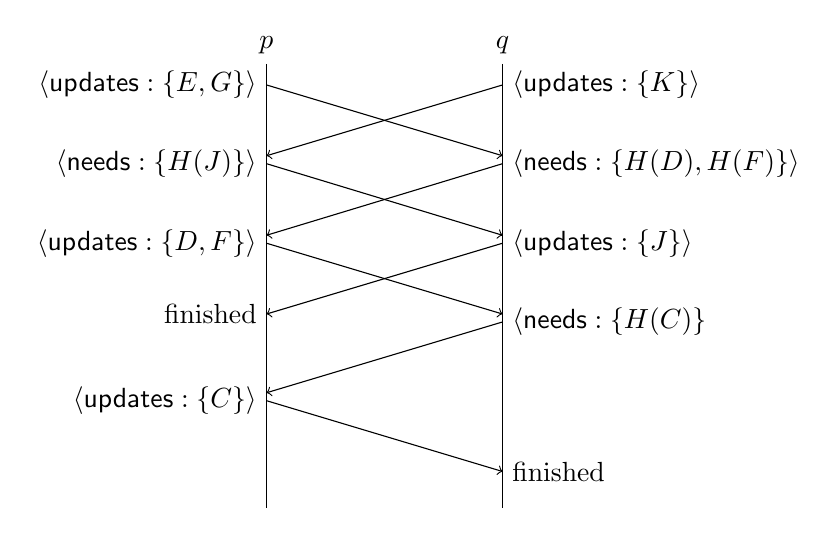
\begin{tikzpicture}
\def\width{3cm}
\def\latency{1cm}
\def\spacing{0.1cm}
\def\length{6cm}
\def\startdelay{0.5cm}

% Timelimes
\node (p1-start) at (0,0) {$p$};
\node (p2-start) at (\width,0) {$q$};
\node (p1-end) at (0,-\length) {};
\node (p2-end) at (\width,-\length) {};
\draw (p1-start) -- (p1-end);
\draw (p2-start) -- (p2-end);

% Messages
\draw[->] (0,-\startdelay) node[left] {$\langle\mathsf{updates}: \{E,G\}\rangle$} -- (\width,\spacing-\startdelay-\latency);
\draw[->] (\width,-\startdelay) node[right] {$\langle\mathsf{updates}: \{K\}\rangle$} -- (0,\spacing-\startdelay-\latency);

\draw[->] (\width, -\startdelay-\latency) node[right] {$\langle\mathsf{needs}: \{H(D), H(F)\}\rangle$} -- (0,\spacing-\startdelay-2.0\latency);
\draw[->] (0, -\startdelay-\latency) node[left] {$\langle\mathsf{needs}: \{H(J)\}\rangle$} -- (\width,\spacing-\startdelay-2.0\latency);

\draw[->] (0, -\startdelay-2.0\latency) node[left] {$\langle\mathsf{updates}: \{D, F\}\rangle$} -- (\width,\spacing-\startdelay-3.0\latency);
\draw[->] (\width, -\startdelay-2.0\latency) node[right] {$\langle\mathsf{updates}: \{J\}\rangle$} -- (0,\spacing-\startdelay-3.0\latency) node[left] {finished};

\draw[->] (\width, -\startdelay-3.0\latency) node[right] {$\langle\mathsf{needs}: \{H(C)\}$} -- (0,\spacing-\startdelay-4.0\latency);

\draw[->] (0, -\startdelay-4.0\latency) node[left] {$\langle\mathsf{updates}: \{C\}\rangle$} -- (\width,\spacing-\startdelay-5.0\latency) node[right] {finished};

\end{tikzpicture}
    \caption{Requests/responses sent in the course of running the reconciliation process in Algorithm~\ref{fig:algorithm} with the example in Figure~\ref{fig:example-dags}.}
    \label{fig:messages}
\end{figure}

We illustrate the operation of the reconciliation algorithm using the example in Figure~\ref{fig:example-dags}; the requests/responses sent in the course of the execution are shown in Figure~\ref{fig:messages}.
Initially, when a connection is established between two processes, they send each other their heads (Algorithm~\ref{fig:algorithm}, line~\ref{line:send-heads}).
In the example of Figure~\ref{fig:example-dags}, $p$ sends $\langle\mathsf{heads}: \{H(E),H(M)\}\rangle$ to $q$, while $q$ sends $\langle\mathsf{heads}: \{H(G),H(K)\}\rangle$ to $p$.

Each process also initialises variables $\mathit{sent}$ and $\mathit{recvd}$ to contain the set of messages sent to/received from the other process within the scope of this particular connection, $\mathit{missing}$ to contain the set of hashes for which we currently lack a message, and $\mathcal{M}_\mathsf{conn}$ to contain a read-only copy of this process' set of messages $\mathcal{M}$ at the time the connection is established (line~\ref{line:init}).
A process may concurrently execute several instances of this algorithm using several connections; each connection then has a separate copy of the variables $\mathit{sent}$, $\mathit{recvd}$, $\mathit{missing}$, and $\mathcal{M}_\mathsf{conn}$, while $\mathcal{M}$ is a global variable that is shared between all connections.
$\mathcal{M}$ should be maintained in stable storage, while the other variables may be lost in case of a crash.

On receiving the heads from the other process (line~\ref{line:recv-heads}), the recipient checks whether the recipient's $\mathcal{M}_\mathsf{conn}$ contains a matching message for each hash.
If any hashes are unknown, it replies with a $\mathsf{needs}$ request for the messages matching those hashes (lines~\ref{line:heads-missing} and \ref{line:send-missing}).
In our running example, $p$ needs $H(G)$, while $q$ needs $H(E)$ and $H(M)$.
A process responds to such a $\mathsf{needs}$ request by returning all the matching messages in a $\mathsf{msgs}$ response (lines~\ref{line:recv-needs}--\ref{line:end-needs}).

On receiving $\mathsf{msgs}$, we first discard any broadcast messages that are not correctly signed by a legitimate process in the system (line~\ref{line:msgs-recvd}).
We then inspect the hashes in each valid message received.
If there are any predecessor hashes that do not resolve to a known message in $\mathcal{M}_\mathsf{conn}$ or $\mathit{recvd}$, we send another $\mathsf{needs}$ request with those hashes (lines~\ref{line:msgs-missing}--\ref{line:msgs-handle-missing}).
In successive rounds of this protocol, the processes work their way from the heads along the paths of predecessors, until they reach the common ancestors of both processes' heads.

Eventually, when there are no unresolved hashes, we perform a topological sort of the graph of received messages to put them in causal order, deliver them to the application, update the global set $\mathcal{M}$ to reflect the messages we have delivered, and conclude the protocol run (lines~\ref{line:missing-empty}--\ref{line:finish}).
We assume that the delivery of messages on line~\ref{line:deliver} and the update of $\mathcal{M}$ on line~\ref{line:update-m} occur atomically.
Once a process completes reconciliation (line~\ref{line:finish}), it can conclude that its current set of delivered messages is a superset of the set of delivered messages on the other process at the start of reconciliation.

When a message $m$ is broadcast, it is also sent as $\langle\mathsf{msgs}: \{m\}\rangle$ on line~\ref{line:eager-send}, and the recipient treats it the same as $\mathsf{msgs}$ received during reconciliation (lines~\ref{line:recv-msgs}--\ref{line:recv-msgs-end}).
Sending messages in this way is not strictly necessary, as the periodic reconciliations will eventually deliver such messages, but broadcasting them eagerly can reduce latency.
Moreover, when a recipient delivers messages, it may also choose to eagerly relay them to other processes it is connected to, without waiting for the next reconciliation (line~\ref{line:eager-relay}); this also reduces latency, but may result in a process redundantly receiving messages that it already has.
The literature on gossip protocols examines in detail the question of when processes should forward messages they receive~\cite{Leitao:2009fi}, while considering trade-offs of delivery latency and bandwidth use; we leave a detailed discussion out of scope for this paper.

We prove in Appendix~\ref{sec:proof} that this algorithm implements all five properties of causal broadcast.
Even though Byzantine-faulty processes may send arbitrarily malformed messages, a correct node will not deliver messages without a complete predecessor graph.
Any messages delivered by one correct node will eventually reach every other correct node through reconciliations.
After reconciliation, both processes have delivered the same set of messages.

\subsection{A more efficient reconciliation algorithm}\label{sec:algorithm2}

A downside of Algorithm~\ref{fig:algorithm} is that the number of round trips can be up to the length of the longest path in the predecessor graph, making it slow when performing reconciliation over a high-latency network.
We now show how to reduce the number of round-trips.

Note that Algorithm~\ref{fig:algorithm} does not store any information about the outcome of the last reconciliation with a particular process; if two processes periodically reconcile their states, they need to discover each other's state from scratch on every protocol run.
As per \S~\ref{sec:system-model} we assume that communication between processes is authenticated, and thus a process knows the identity of the other process it is communicating with.
We can therefore record the outcome of a protocol run with a particular process, and use that information in the next reconciliation with the same process.
We do this by adding the following instruction after line~\ref{line:update-m} of Algorithm~\ref{fig:algorithm}, where $q$ is the identity of the current connection's remote process:
\[ \textsc{StoreHeads}(q, \mathrm{heads}(\mathcal{M}_\mathsf{conn} \cup \mathit{recvd})) \]
which updates a key-value store in stable storage, associating the value $\mathrm{heads}(\mathcal{M}_\mathsf{conn} \cup \mathit{recvd})$ with the key $q$ (overwriting any previous value for that key if appropriate).
We use this information in Algorithm~\ref{fig:algorithm2}, which replaces the ``on connecting'' and ``on receiving heads'' functions of Algorithm~\ref{fig:algorithm}, while leaving the rest of Algorithm~\ref{fig:algorithm} unchanged.

\begin{algorithm}[t]
    \begin{algorithmic}[1]
    \On{connecting to process $q$}\Comment{Replaces lines \ref{line:connect-begin}--\ref{line:connect-end} of Algorithm \ref{fig:algorithm}}
        \State $\mathit{sent} := \{\};\; \mathit{recvd} := \{\};\; \mathit{missing} := \{\};\; \mathcal{M}_\mathsf{conn} := \mathcal{M}$ \Comment{connection-local variables}
        \State $\mathit{oldHeads} := \Call{LoadHeads}{q}$\label{line:load-heads}
        \State $\mathit{filter} := \textsc{MakeBloomFilter}(\Call{MessagesSince}{\mathit{oldHeads}})$\label{line:make-bloom}
        \State \textbf{send} $\langle\mathsf{heads}: \mathrm{heads}(\mathcal{M}_\mathsf{conn}),\, \mathsf{oldHeads}: \mathit{oldHeads},\, \mathsf{filter}: \mathit{filter}\rangle$ \label{line:a2-send-heads}
    \EndOn
    \State
    \On{receiving $\langle\mathsf{heads}: \mathit{hs},\, \mathsf{oldHeads}: \mathit{oldHeads},\, \mathsf{filter}: \mathit{filter}\rangle$}\Comment{Replaces lines \ref{line:recv-heads}--\ref{line:recv-heads-end}}\label{line:a2-recv-heads}
        \State $\mathit{bloomNegative} := \{m \in \Call{MessagesSince}{\mathit{oldHeads}} \mid \neg\Call{BloomMember}{\mathit{filter}, m}\}$\label{line:bloom-member}
        \State $\mathit{reply} := \left(\mathit{bloomNegative} \,\cup\, \bigcup_{m \in \mathit{bloomNegative}} \mathrm{succ}^*(\mathcal{M}_\mathsf{conn}, m)\right) \setminus \mathit{sent}$\label{line:bloom-succ}
        \If{$\mathit{reply} \neq \{\}$}
            \State $\mathit{sent} := \mathit{sent} \cup \mathit{reply}$
            \State \textbf{send} $\langle\mathsf{msgs}: \mathit{reply}\rangle$ \label{line:a2-heads-reply}
        \EndIf
        \State \Call{HandleMissing}{$\{h \in \mathit{hs} \mid \nexists m \in \mathcal{M}_\mathsf{conn}.\; H(m) = h\}$} \label{line:a2-heads-missing}
    \EndOn
    \State
    \Function{MessagesSince}{$\mathit{oldHeads}$}\label{line:msg-since-begin}
        \State $\mathit{known} := \{m \in \mathcal{M}_\mathsf{conn} \mid H(m) \in \mathit{oldHeads}\}$
        \State \textbf{return} $\mathcal{M}_\mathsf{conn} \setminus \left(\mathit{known} \,\cup\, \bigcup_{m \in \mathit{known}} \mathrm{pred}^*(\mathcal{M}_\mathsf{conn}, m)\right)$
    \EndFunction\label{line:msg-since-end}
    \end{algorithmic}
    \caption{Optimising Algorithm~\ref{fig:algorithm} to reduce the number of round-trips.}\label{fig:algorithm2}
\end{algorithm}

First, when process $p$ establishes a connection with process $q$, $p$ calls $\textsc{LoadHeads}(q)$ to load the heads from the previous reconciliation with $q$ from the key-value store (Algorithm~\ref{fig:algorithm2}, line~\ref{line:load-heads}).
This function returns the empty set if this is the first reconciliation with $q$.
In the example of Figure~\ref{fig:example-dags}, the previous reconciliation heads might be $\{H(B)\}$.

In lines~\ref{line:msg-since-begin}--\ref{line:msg-since-end} we find all of the delivered messages that were added to $\mathcal{M}$ since this last reconciliation (i.e.\ all messages that are not among the last reconciliation's heads or their predecessors), and construct a Bloom filter~\cite{Bloom:1970} containing those messages.
In the example of Figure~\ref{fig:example-dags}, $p$'s Bloom filter would contain $\{C, D, E, J, K, L, M\}$, while $q$'s filter contains $\{F, G, J, K\}$.
We send this Bloom filter to the other process, along with the heads (lines~\ref{line:make-bloom}--\ref{line:a2-send-heads}).

On receiving the heads and Bloom filter, we identify any messages that were added since the last reconciliation that are \emph{not} present in the Bloom filter's membership check (line~\ref{line:bloom-member}).
In the example, $q$ looks up $\{F, G, J, K\}$ in the Bloom filter received from $p$; \textsc{BloomMember} returns true for $J$ and $K$. For $F$ and $G$, \textsc{BloomMember} is likely to return false, but may return true.
In this example we assume that the Bloom membership check returns false for $F$ and true for $G$ (a false positive in the case of $G$).

Any Bloom-negative messages are definitely unknown to the other process, so we send those in reply.
Moreover, we also send any successors of Bloom-negative messages (line~\ref{line:bloom-succ}): since the set $\mathcal{M}$ for a correct process cannot contain messages whose predecessors are missing, we know that these messages must also be missing from the other process.
In the example, $q$ sends $\langle\mathsf{msgs}: \{F, G\}\rangle$ to $p$, because $F$ is Bloom-negative and $G$ is a successor of $F$.

Due to Bloom filter false positives, the set of messages in the reply on line~\ref{line:a2-heads-reply} may be incomplete, but it is likely to contain most of the messages that the other process is lacking.
To fill in the remaining missing messages we revert back to Algorithm~\ref{fig:algorithm}, and perform round trips of $\mathsf{needs}$ requests and $\mathsf{msgs}$ responses until the received set of messages is complete.

The size of the Bloom filter can be chosen dynamically based on the number of elements it contains.
Note that the Bloom filter reflects only messages that were added since the last reconciliation with $q$, not all messages $\mathcal{M}$.
Thus, if the reconciliations are frequent, they can employ a small Bloom filter size to minimise the cost of reconciliation.

This optimised algorithm also tolerates Byzantine faults.
For example, a faulty replica may send a correct replica an arbitrarily corrupted Bloom filter, but this only changes the set of messages in the reply from the correct process, and has no effect on $\mathcal{M}$ at the correct process.
We formally analyse the correctness of this algorithm in Appendix~\ref{sec:proof}.

\subsection{Discussion}

A potential issue with Algorithms~\ref{fig:algorithm} and~\ref{fig:algorithm2} is the unbounded growth of storage requirements, since the set $\mathcal{M}$ grows monotonically (much like most algorithms for Byzantine agreement, which produce an append-only log without considering how that log might be truncated).
Since the set of processes in the system is known, we can truncate history as follows: once every process has delivered a message $m$ (i.e.\ $m$ is \emph{stable}~\cite{Birman:1991el}), the algorithm no longer needs to refer to any of the predecessors of $m$, and so all of those predecessors can be safely removed from $\mathcal{M}$ without affecting the algorithm.
Stability can be determined by keeping track of the latest heads for each process, and propagating this information between processes.

When one of the communicating processes is Byzantine-faulty, the reconciliation algorithm may never terminate, e.g.\ because the faulty process may send hashes that do not resolve to any message, and so the state $\mathit{missing} = \{\}$ is never reached.
However, in a non-terminating protocol run no messages are delivered and $\mathcal{M}$ is never updated, and so the actions of the faulty process have no effect on the state of the correct process.
Reconciliations with other processes are unaffected, since processes may perform multiple reconciliations concurrently.

In a protocol run that terminates, the only possible protocol violations from a Byzantine-faulty process are to omit heads, or to extend the set $\mathcal{M}$ with well-formed messages (i.e.\ messages containing only hashes that resolve to other messages, signed with the private key of one of the processes in the system).
Any omitted messages will eventually be received through reconciliations with other correct processes, and any added messages will be forwarded to other processes; either way, the eventual delivery property of causal broadcast is preserved.

Arbitrary $\mathsf{needs}$ requests sent by a faulty process have no consequence, since they do not affect the state of the recipient.
Thus, a faulty process cannot corrupt the state of a correct process in a way that would prevent it from later reconciling with another correct process.

If message loss occurs during reconciliation, the connection times out and no messages are delivered.
The next reconciliation attempt then starts afresh.
Note also that it is possible for one process in a connection to complete reconciliation while the other times out and aborts, due to one-sided message loss.
Thus, when we load the heads from the previous reconciliation on line~\ref{line:load-heads} of Algorithm~\ref{fig:algorithm2}, the local and the remote process' $\mathit{oldHeads}$ may differ.
This does not affect the correctness of the algorithm.

\begin{figure}
  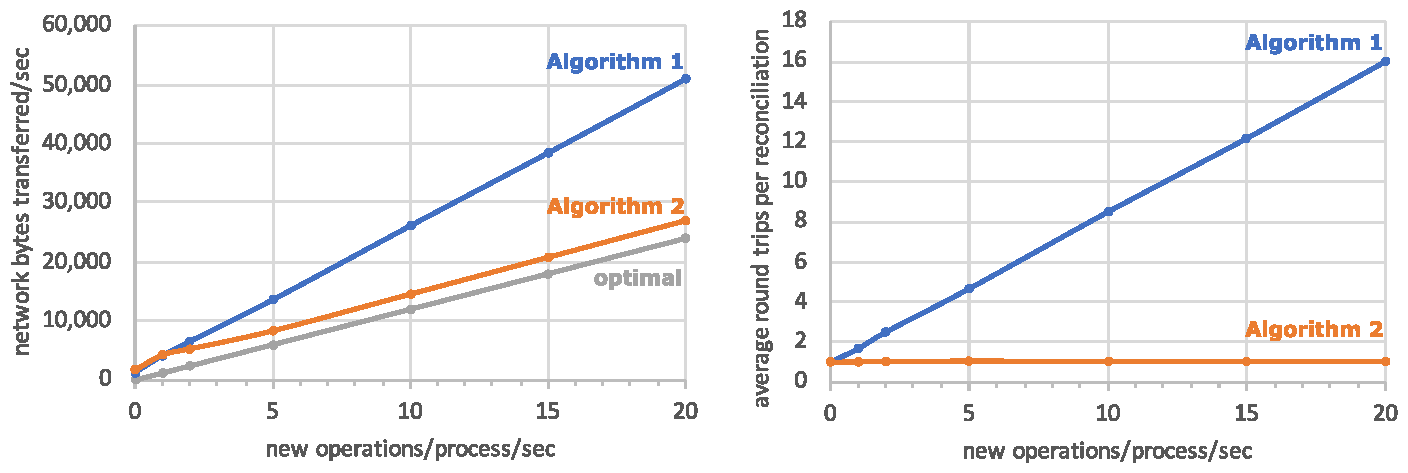
\includegraphics[width=\textwidth,keepaspectratio=true]{figs/evaluation.pdf}
  \caption{left: number of round trips until reconciliation is complete; right: network bandwidth used to reconcile four processes once per second (lower is better).}
  \label{fig:evaluation}
\end{figure}

\subsection{Evaluation}\label{sec:evaluation}

To evaluate the algorithms introduced in \S~\ref{sec:algorithm1} and \S~\ref{sec:algorithm2} we implemented both algorithms and measured their behaviour in a simulated network.
In our experiments we use four processes, where every pair of processes reconciles their states once per second.
Each process concurrently broadcasts new messages, and we vary the rate at which new messages are broadcast.
To ensure we exercise the reconciliation algorithm, processes do not eagerly send messages (lines~\ref{line:eager-send} and~\ref{line:eager-relay} of Algorithm~\ref{fig:algorithm} are omitted), and we rely only on periodic reconciliation to exchange messages.
% 6 pairwise reconciliations take place every second

First, we measure the average number of round-trips required to complete one reconciliation (Figure~\ref{fig:evaluation} left).
The higher the rate of broadcasts, the longer the paths in the predecessor graph.
Therefore, when Algorithm~\ref{fig:algorithm} is used, the number of round trips increases linearly with the rate at which messages are broadcast.
However, Algorithm~\ref{fig:algorithm2} reduces each reconciliation to 1.03 round trips on average, and this number remains constant as the rate of broadcasts grows.
97\% of reconciliations complete in one round trip, while only 2.9\% require two round trips, and 0.02\% of reconciliations require three or more round trips.
These figures are based on using Bloom filters with 10 bits per entry and 7 hash functions.

Next, we estimate the network traffic resulting from the use of our algorithms.
For this we assume that each broadcast message is 400 bytes in size (not counting its predecessor hashes), hashes are 32 bytes in size (as in SHA-256), and Bloom filters use 10 bits per element.
Moreover, we assume that each request or response incurs an additional constant overhead of 50 bytes (e.g.\ for TCP/IP packet headers and signatures).
We compute the number of kilobytes sent per second (in both directions) using each reconciliation algorithm.

Figure~\ref{fig:evaluation} (right) shows the results from this experiment.
The grey line represents a hypothetical optimal algorithm that transmits only new messages, but no additional metadata such as hashes or Bloom filters.
Compared to this optimum, Algorithm~\ref{fig:algorithm2} incurs a near-constant overhead of approximately 800 bytes per reconciliation for the heads and predecessor hashes, Bloom filter, and occasional additional round trips.
In contrast, Algorithm~\ref{fig:algorithm} incurs an approximately 40\% overhead, primarily because it sends many $\mathsf{needs}$ messages containing hashes, and it sends messages in many small responses rather than batched into one response.

Thus, we can see that in terms of network performance, Algorithm~\ref{fig:algorithm2} is close to the optimum of one round trip, and incurs only a small overhead in terms of bytes transmitted.
We leave an evaluation of other metrics (e.g.\ CPU or memory use) for future work.

\section{Implementing replicated storage using causal broadcast}\label{sec:byzantine-crdts}

Eventual consistency is usually defined as: ``If no further updates are made, then eventually all replicas will be in the same state~\cite{Vogels:2009ca}.''
This is a very weak model: it does not specify when the consistent state will be reached, and the premise ``if no further updates are made'' may never be true in a system in which updates happen continuously.
To strengthen this model, Shapiro et al.~\cite{Shapiro:2011} introduce \emph{strong eventual consistency} (SEC), which requires that:

\begin{description}
\item[Eventual update:] If an update is applied by a correct replica, then all correct replicas will eventually apply that update.
\item[Convergence:] Any two correct replicas that have applied the same set of updates are in the same state (even if the updates were applied in a different order).
\end{description}

Strong eventual consistency (SEC) is defined in a non-Byzantine system model.
Replicated storage systems with SEC can be implemented using \emph{Conflict-free Replicated Data Types} (\emph{CRDTs})~\cite{Shapiro:2011}.
These are data structures that can be concurrently modified on multiple replicas without any locking or other synchronous coordination, even while offline.
Whenever a replica updates its copy of the shared data, operation-based CRDTs capture this update as an \emph{operation}, encode it as a message, and broadcast it to the other replicas.

Operation-based CRDTs typically use causal broadcast to disseminate operations to all replicas~\cite{Gomes:2017gy,Shapiro:2011}.
The CRDT is designed such that concurrent (causally unrelated) operations are commutative, i.e.\ they can be applied in any order without affecting the final state.
Thus, no matter in which order the causal broadcast protocol delivers messages, convergence is assured.
For space reasons we elide a detailed discussion of how CRDTs achieve this commutativity for different types of data structures, and we refer the interested reader to extensive discussions of this topic in the CRDT literature~\cite{Gomes:2017gy,Shapiro:2011wy,Weiss:2009ht}.

CRDTs can replicate data in generic data models such as key-value stores~\cite{Akkoorath2016Cure,Zawirski2015SwiftCloud} and relational databases, as well as various other datatypes: there are CRDT-based multi-user collaborative text editors~\cite{Weiss:2009ht}, note-taking tools~\cite{vanHardenberg2020PushPin}, games~\cite{vanderLinde:2017fu}, CAD applications~\cite{Lv:2018ie}, distributed filesystems~\cite{Najafzadeh:2018bw,Tao:2015gd}, project management tools~\cite{Kleppmann2019localfirst}, and many other applications.
The SEC properties of several CRDTs has been formally verified~\cite{Gomes:2017gy,Zeller:2014fl}.

\subsection{Defining and implementing Byzantine Eventual Consistency}

We say a replicated storage system provides Byzantine Eventual Consistency (BEC) if it satisfies the following properties in the Byzantine system model of \S~\ref{sec:system-model}:

\begin{description}
\item[Validity:] If a correct replica applies an update that is labelled as originating from process $s$, then that update was generated by process $s$.
\item[Non-duplication:] A correct replica does not apply the same update more than once.
\item[Self-update:] If a correct replica generates an update, it applies that update to its own state.
\item[Eventual update:] For any update applied by a correct replica, all correct replicas will eventually apply that update.
\item[Causal consistency:] If a correct replica generates or applies update $u_1$ before generating update $u_2$, then all replicas apply $u_1$ before $u_2$.
\item[Convergence:] Any two correct replicas that have applied the same set of updates are in the same state.
\end{description}

BEC is a slight strengthening of SEC; the main difference is that SEC assumes a non-Byzantine system~\cite{Shapiro:2011}, and SEC does not explicitly require causal consistency (even though many CRDTs provide this property anyway).
Unlike Byzantine agreement (\S~\ref{sec:relwork}), BEC is not strong enough to implement a cryptocurrency, since it cannot prevent double-spending.
However, it is sufficient for many applications that currently use CRDTs.

We can implement BEC replicated state using Byzantine causal broadcast (\S~\ref{sec:algorithm}) and operation-based CRDTs.
Whenever a replica wishes to update the state of a CRDT, it generates an \emph{operation} describing that update, encodes that operation as a message, and sends it to the other replicas via Byzantine causal broadcast.
On delivering that message, each replica (including the sender) applies the operation to its local CRDT state.
Each operation has a unique logical timestamp as specified below.
The first five properties of BEC then follow immediately from the five properties of causal broadcast~\cite{Gomes:2017gy}.

The CRDT algorithm ensures that concurrent operations commute: thus, any operations whose order is left ambiguous by the \emph{causal order} property of causal broadcast can be applied in any order without affecting the final state.
On the other hand, any operations that are predecessors or successors of one another need not be commutative, since causal broadcast will deliver them in the same order at each replica.
Hence we obtain the \emph{convergence} property.

In addition to causal broadcast, many CRDT algorithms require that each operation has a globally unique logical timestamp.
For example, in a last-writer-wins register, if several replicas concurrently write to the register, then the merged final value of the register is the value written by the operation with the greatest logical timestamp~\cite{Shapiro:2011wy}.

When using our causal broadcast algorithms from \S~\ref{sec:algorithm} we can assign such timestamps as follows.
For every message $m$ let the logical timestamp $T(m)$ of that message be:
\[ T(m) = 0 \quad\text{if } \mathrm{pred}^1(m) = \{\}, \qquad
T(m) = 1 + \max_{m' \in \mathrm{pred}^1(m)} T(m') \quad\text{otherwise.} \]
We define a total order lexicographically by breaking ties using the message hash:
\[ m_1 < m_2 \iff (T(m_1) < T(m_2) \;\vee\; (T(m_1) = T(m_2) \,\wedge\, H(m_1) < H(m_2)). \]
This construction is similar to Lamport timestamps~\cite{Lamport:1978}: a successor always has a greater timestamp than its predecessors, making the timestamp order a linear extension of the causal order.
Since we assume that the hash function is collision-free, the (timestamp, hash) pair for a message/operation is globally unique, as required by CRDTs.

\section{Related Work}\label{sec:relwork}

Byzantine agreement has been subject of extensive research and has seen a recent renewal of interest due to its application in permissioned blockchains~\cite{Bano:2019}.
To tolerate $f$ faults, Byzantine agreement algorithms typically require $3f+1$ processes~\cite{Castro:1999,Kotla:2007,Bessani:2014}, and some even require $5f+1$ processes~\cite{Abd:2005,Martin:2006}.
Some algorithms instead take a different approach to bounding the number of failures: for example, Upright~\cite{Clement:2009} separates the number of crash failures ($u$) and Byzantine failures ($r$) and uses $2u+r+1$ processes.
% Most algorithms also require at least one round of communication with at least $2f+1$ processes, incurring both significant latency and limiting availability.
Zeno~\cite{Singh:2009} makes progress with just $f+1$ processes, but safety depends on less than $\frac{1}{3}$ of processes being Byzantine-faulty.
Previous work on Byzantine fault tolerant CRDTs~\cite{Chai:2014,Shoker:2017,Zhao:2016}, Secure Causal Atomic Broadcast~\cite{Cachin:2001cj,Duan:2017} and Byzantine Lattice Agreement~\cite{DiLuna:2020} also assumes $3f+1$ processes.

In SPORC~\cite{Feldman:2010wl}, BFT2F~\cite{Li:2007} and SUNDR~\cite{Mazieres:2002}, a faulty process can partition the system, preventing some processes from ever synchronising again, so these systems do not satisfy the \emph{eventual update} property of BEC.
Depot~\cite{Mahajan:2011} and OldBlue~\cite{VanGundy:2012} provide causal broadcast while tolerating arbitrary numbers of faulty processes.
OldBlue's algorithm is similar to our Algorithm~\ref{fig:algorithm}, while Depot uses a more complex algorithm that is not precisely specified, involving both version vectors and hash chains.
Depot's consistency model (fork-join-causal) is considerably more complicated than BEC, and it is unclear which is more useful in practice.

Beyond the field of Byzantine fault tolerance, the problems of computing the difference, union or intersection between sets on remote hosts has been studied in various domains, including peer-to-peer systems, deduplication of backups, and error-correction.
Approaches include using Bloom filters~\cite{Skjegstad:2011} similar to Algorithm 2, invertible Bloom filters~\cite{Goodrich:2011,Eppstein:2011} and polynomial encoding~\cite{Minsky:2006}.
These approaches are not designed to tolerate Byzantine faults.

Snapdoc~\cite{Kollmann:2019hf} has previously examined cryptographic integrity checks for CRDTs, but its approach (using RSA accumulators) incurs large overheads.
Truong et al.~\cite{Truong:2012et} present another scheme for authenticating CRDT history, but do not include a reconciliation protocol.

Hash chaining is widely used: in blockchains~\cite{Bano:2019}, Git commit histories, Merkle trees~\cite{Merkle:1987}, and peer-to-peer storage systems such as IPLD~\cite{IPLD}.
Our Algorithm~\ref{fig:algorithm} has similarities to the protocol used by \texttt{git fetch}~\cite{GitHTTP}.
Other authors~\cite{Baird:2016tq,Kang:2003} also discuss replicated hash graphs, but don't present efficient reconcilation algorithms.

% Tseng et al.~\cite{Tseng:2019jb} prove that Byzantine causal memory can only be done with $3f+1$ processes?!

% https://github.com/sipa/minisketch

% Merkle clocks https://hector.link/presentations/merkle-crdts/merkle-crdts.pdf

% Roy Friedman and Roni Licher. Hardening Cassandra Against Byzantine Failures.
% https://arxiv.org/pdf/1610.02885.pdf

% Git fetch negotiation algorithm, How does this compare to git fetch negotiation algorithms, default and skipping?  
% https://stackoverflow.com/questions/40484929/will-a-git-pull-develop-fetch-all-the-commits-reacheable-from-develop
% https://git-scm.com/docs/git-config#Documentation/git-config.txt-fetchnegotiationAlgorithm

% Comparison to Julien Quintard work on byzantine file systems https://www.repository.cam.ac.uk/bitstream/handle/1810/243442/thesis.pdf?sequence=1&isAllowed=y
% https://infinit.sh

% Comparison to irmin
% https://mirage.github.io/irmin/irmin/Irmin/index.html#syncing-with-a-remote
% https://github.com/mirage/irmin/blob/master/src/irmin/sync_ext.ml#L86-L123

% Comparision to byzantine quorums
% http://www.cs.cornell.edu/courses/cs5414/2017fa/papers/bquorum-dc.pdf

% Comparision to byz chain replication
% https://link.springer.com/chapter/10.1007/978-3-642-35476-2_24

\section{Conclusions}

Some systems, e.g.\ peer-to-peer Internet applications, need to tolerate arbitrary numbers of Byzantine-faulty processes and are thus not suitable applications for Byzantine agreement.
In this paper, we have defined Byzantine Eventual Consistency (BEC), a consistency model that can be achieved regardless of the number of Byzantine-faulty processes in a system, and without making any synchrony assumptions.
We have proposed reconciliation algorithms that implement Byzantine causal broadcast, proved their correctness, and evaluated their performance.
Our optimised algorithm incurs only a small network communication overhead compared to the theoretical optimum, making it immediately applicable in practice.

As shown in \S~\ref{sec:byzantine-crdts}, many existing systems and applications use CRDTs to achieve strong eventual consistency in a non-Byzantine model.
Adopting our approach will allow those systems to gain robustness against Byzantine faults without significant changes to their existing CRDT algorithms.
For systems that currently require all nodes to be trusted, and hence can only deployed in trusted datacenter networks, adding Byzantine fault tolerance opens up new opportunities for deployment in untrusted settings, e.g.\ on the public Internet.

We hope that BEC will inspire further research to ensure the correctness of eventually consistent systems in the presence of arbitrary numbers of Byzantine faults.

\bibliographystyle{plainurl}
\bibliography{references}
\newpage\appendix

\section{Proof of correctness}\label{sec:proof}

In this section we show that Algorithms~\ref{fig:algorithm} and \ref{fig:algorithm2} implement causal broadcast, as defined in \S~\ref{sec:background}, in the Byzantine system model of \S~\ref{sec:system-model}.
If a lemma does not specify which of the two algorithms it applies to, it holds for both.

\begin{lemma}\label{lemma:easy-properties}
Algorithms~\ref{fig:algorithm} and \ref{fig:algorithm2} satisfy the \emph{validity}, \emph{non-duplication}, \emph{self-delivery}, and \emph{causal order} properties of causal broadcast.
\end{lemma}
\begin{proof}
The \emph{validity} property holds because when a broadcast message is delivered, it was either sent by the local process, or it was received from another process in a reconciliation.
In the latter case, messages are in the set $\mathcal{M}$ only if they were broadcast, and we discard any messages that do not have a valid signature from a process in the system (Algorithm~\ref{fig:algorithm}, line~\ref{line:msgs-recvd}).
Thus, in either case, a correct process delivers a message only if it was broadcast by a process.

The \emph{non-duplication} property holds because newly broadcast messages are assumed to be unique, and messages delivered during reconciliation are limited to those not already in $\mathcal{M}$ (Algorithm~\ref{fig:algorithm}, line~\ref{line:deliver}).
Since $\mathcal{M}$ is immediately updated to include all delivered messages, this ensures that no correct process delivers the same message more than once.

The \emph{self-delivery} property holds trivially, because we assume that whenever a correct process broadcasts a message, it immediately delivers that message to itself.

The \emph{causal order} property holds because when a correct process broadcasts a message, the predecessor hashes are computed such that every message previously broadcast or delivered by this process becomes a (direct or indirect) predecessor of the new message.
Any correct process delivers messages in topologically sorted order, i.e.\ any predecessors of $m$ are delivered before $m$.
The reconciliation algorithm delivers messages only once all hashes have been resolved (once all direct and indirect predecessor messages have been received), so we know that there are no missing predecessors.
Thus, whenever a correct process broadcasts or delivers $m_1$ before broadcasting $m_2$, all correct processes deliver $m_1$ before delivering $m_2$.
\end{proof}

This leaves the \emph{eventual delivery} property, which is the focus of the remainder of this appendix.
We consider two correct processes $p$ and $q$, with initial sets of messages $\mathcal{M}_p$ and $\mathcal{M}_q$ respectively at the start of the execution.
Assume that in this run of the algorithm, $p$ and $q$ both complete the reconciliation by reaching line~\ref{line:finish} of Algorithm~\ref{fig:algorithm}.
Let $\mathit{recvd}_p$ be the contents of the variable $\mathit{recvd}$ at process $p$ when the reconciliation is complete, and likewise $\mathit{recvd}_q$ at process $q$.
Further, let $\mathcal{M}'_p = \mathcal{M}_p \cup \mathit{recvd}_p$ and $\mathcal{M}'_q = \mathcal{M}_q \cup \mathit{recvd}_q$ be the final set of messages at both processes.

\begin{lemma}\label{lemma:no-p-missing}
The set of messages $\mathcal{M}$ of a correct process $p$ grows monotonically.
\end{lemma}
\begin{proof}
The process $p$ only modifies $\mathcal{M}$ by unioning it with the set $\mathit{recvd}$ (Algorithm~\ref{fig:algorithm}, line~\ref{line:update-m}), or by generating new operations, which are added to $\mathcal{M}$.
Thus, elements are only added to the set $\mathcal{M}$, and therefore $\mathcal{M}$ grows monotonically.
\end{proof}

\begin{lemma}\label{lemma:no-dangling}
Let $m = (v, \mathit{hs}, \mathit{sig})$ and $m \in \mathcal{M}_p$.
Then $\forall h \in \mathit{hs}.\; \exists m' \in \mathcal{M}_p.\; H(m') = h$.
\end{lemma}
\begin{proof}
There are two ways how $m$ can become a member of $\mathcal{M}_p$ for a correct process $p$:
\begin{enumerate}
    \item $m$ is broadcast by process $p$.
    In this case, since $p$ is assumed to be correct, the hashes $\mathit{hs}$ are computed as $\mathit{hs} = \{H(m') \mid m' \in \mathcal{M} \wedge \mathrm{succ}^1(\mathcal{M}, m') = \{\}\,\}$ for some earlier state $\mathcal{M}$ (Algorithm~\ref{fig:algorithm}, line~\ref{line:broadcast-heads}).
    As $\mathcal{M}$ grows monotonically (Lemma~\ref{lemma:no-p-missing}), $\mathcal{M} \subseteq \mathcal{M}_p$, and thus we can deduce that $\forall h \in \mathit{hs}.\; \exists m' \in \mathcal{M}_p.\; H(m') = h$.
    \item $m$ is received from another process (which might be faulty).
    In this case, during the run of the protocol at which $p$ received $m$, we have $m \in \mathit{recvd}$ and $\mathit{missing} = \{\}$ at line~\ref{line:update-m} of Algorithm~\ref{fig:algorithm}.
    Let $\mathcal{M}$ be the set of messages at $p$ immediately before that execution of line~\ref{line:update-m}.
    From $\mathit{missing} = \{\}$ and line~\ref{line:msgs-missing} of Algorithm~\ref{fig:algorithm} we can deduce that $\forall h \in \mathit{hs}.\; \exists m' \in (\mathcal{M} \cup \mathit{recvd}).\; H(m') = h$.
    Since $\mathcal{M}$ grows monotonically (Lemma~\ref{lemma:no-p-missing}) and $\mathit{recvd} \subseteq \mathcal{M}_p$ (line~\ref{line:update-m}) we have $\forall h \in \mathit{hs}.\; \exists m' \in \mathcal{M}_p.\; H(m') = h$.
\end{enumerate}
\end{proof}

\begin{lemma}\label{lemma:no-collision}
Let $m = (v, \mathit{hs}, \mathit{sig})$ such that $m \in \mathcal{M}_p$ and $m \in \mathcal{M}_q$.
Then the hashes $\mathit{hs}$ resolve to the same messages at $p$ and $q$, i.e.\ $\{m' \in \mathcal{M}_p \mid H(m') \in \mathit{hs}\} = \{m' \in \mathcal{M}_q \mid H(m') \in \mathit{hs}\}$.
\end{lemma}
\begin{proof}
We use proof by contradiction.\\
Assume there exists $h \in \mathit{hs}$ such that $\{m' \in \mathcal{M}_p \mid H(m') = h\} \neq \{m' \in \mathcal{M}_q \mid H(m') = h\}$.\\
By Lemma~\ref{lemma:no-dangling} we have $\{m' \in \mathcal{M}_p \mid H(m') = h\} \neq \{\}$ and $\{m' \in \mathcal{M}_q \mid H(m') = h\} \neq \{\}$.\\
Hence, there exist $m' \in \mathcal{M}_p$ and $m'' \in \mathcal{M}_q$ such that $m' \neq m''$ and $H(m') = H(m'') = h$.\\
However, this contradicts our assumption in \S~\ref{sec:algorithm} that the hash function $H(\cdot)$ is collision-resistant.
\end{proof}

\begin{lemma}\label{lemma:no-q-missing}
$\mathcal{M}_q \subseteq \mathcal{M}'_p$ when executing Algorithm~\ref{fig:algorithm}.
\end{lemma}
\begin{proof}
We use proof by contradiction.\\
Assume that $\exists m \in \mathcal{M}_q.\; m \notin  \mathcal{M}'_p$.\\
Since $\mathit{recvd} \subseteq \mathcal{M}'_p$ and elements are only added to $\mathit{recvd}$ (Algorithm~\ref{fig:algorithm}, line~\ref{line:msgs-recvd}) then $m \notin  \mathcal{M}'_p$ implies that $m \notin \mathit{recvd}$ on process $p$.\\
Since $m \in \mathcal{M}_q$ we have either $\mathrm{succ}^1(\mathcal{M}_q, m) = \{\}$ or $\mathrm{succ}^1(\mathcal{M}_q, m) \ne \{\}$, and we now consider each case in turn.
\begin{enumerate}
    \item\textsc{Case} $\mathrm{succ}^1(\mathcal{M}_q, m) = \{\}$:\\
    In this case, $H(m) \in \mathrm{heads}(\mathcal{M}_q)$, and so the first $\mathsf{heads}$ request from $q$ to $p$ will contain $H(m)$ (Algorithm~\ref{fig:algorithm}, line~\ref{line:send-heads}).\\
    Since $m \notin \mathcal{M}_p$, process $p$ will send a $\mathsf{needs}$ request to $q$ containing $H(m)$ (Algorithm~\ref{fig:algorithm}, line~\ref{line:heads-missing}).\\
    Upon receiving the $\mathsf{needs}$ message containing $H(m)$, process $q$ will reply with an $\mathsf{msgs}$ response containing $m$ (Algorithm~\ref{fig:algorithm}, line~\ref{line:send-msgs}).\\
    Process $p$ will receive the $\mathsf{msgs}$ response with $m$ from process $q$ and will add $m$ to $\mathit{recvd}$ (Algorithm~\ref{fig:algorithm}, line~\ref{line:msgs-recvd}).\\
    This contradicts our previous finding that $m \notin \mathit{recvd}$.
    
    \item\textsc{Case} $\mathrm{succ}^1(\mathcal{M}_q, m) \ne \{\}$:\\
    In this case, $H(m) \notin \mathrm{heads}(\mathcal{M}_q)$.
    Since $\mathcal{M}_q$ is a DAG, there must exist a message $m'$ such that $H(m') \in \mathrm{heads}(\mathcal{M}_q)$ and $m' \in \mathrm{succ}^*(\mathcal{M}_q, m)$.\\
    As in the previous case, $H(m') \in \mathrm{heads}(\mathcal{M}_q)$ implies that $m' \in \mathit{recvd}$.\\
    Note that none of the messages in $\mathrm{succ}^*(\mathcal{M}_q, m)$ are in $\mathcal{M}_p$ as $m \notin \mathcal{M}'_p$ implies that  $m \notin \mathcal{M}_p$ (Lemma~\ref{lemma:no-p-missing}).\\
    If $m' \in \mathrm{succ}^1(\mathcal{M}_q, m)$ then it must the case that $m \in \mathit{recvd}$ by the time that $\mathit{missing} = \emptyset$, otherwise $m \in \mathit{missing}$ (Algorithm~\ref{fig:algorithm}, line~\ref{line:msgs-missing}).\\
    By induction over the path of successors from $m'$ to $m$, we observe that $m \in \mathit{recvd}$.\\
    At each step of the induction, the processes move to the predecessors of the previous step; due to Lemma~\ref{lemma:no-collision}, $p$ and $q$ agree about the identity of these predecessors.\\
    This contradicts our previous finding that $m \notin \mathit{recvd}$.
\end{enumerate}
\end{proof}

\begin{lemma}\label{lemma:no-q-missing2}
$\mathcal{M}_q \subseteq \mathcal{M}'_p$ when executing Algorithm~\ref{fig:algorithm2}.
\end{lemma}
\begin{proof}
By contradiction.
Assume $m \in \mathcal{M}_q$, $m \notin \mathcal{M}_p'$ and $m \notin \mathit{recvd}$ like in Lemma~\ref{lemma:no-q-missing}.\\
Let $\mathit{filter}$ be the Bloom filter in the initial message from $p$ to $q$ in the current protocol run.\\
Even though we have $m \notin \mathcal{M}_p$ (by Lemma~\ref{lemma:no-p-missing}), $\textsc{BloomMember}(\mathit{filter}, m)$ may return a false positive.
Moreover, if it returns true, $m$ may or may not be a successor of a $\mathit{bloomNegative}$ item as computed in Algorithm~\ref{fig:algorithm2}, lines~\ref{line:bloom-member}--\ref{line:bloom-succ}.\\
As a result it is possible for either $m \in \mathit{reply}$ or $m \notin \mathit{reply}$ after executing line~\ref{line:bloom-succ}.\\
If $m \in \mathit{reply}$ then $p$ will receive an $\mathsf{msgs}$ response containing $m$, which will be added to $\mathit{recvd}$, contradicting our assumption that $m \notin \mathit{recvd}$.\\
If $m \notin \mathit{reply}$ we continue to line~\ref{line:a2-heads-missing} of Algorithm~\ref{fig:algorithm2}, from which point onward the algorithm is the same as Algorithm~\ref{fig:algorithm}.
Thus, we have $\mathcal{M}_q \subseteq \mathcal{M}'_p$ by Lemma~\ref{lemma:no-q-missing}.
\end{proof}

\begin{lemma}\label{lemma:no-extras}
$\mathcal{M}'_p \subseteq \mathcal{M}_p \cup \mathcal{M}_q$.
\end{lemma}
\begin{proof}
We use proof by contradiction.\\
Assume that $\exists m \in \mathcal{M}'_p.\; m \notin \mathcal{M}_p  \land  m \notin \mathcal{M}_q$.\\
Since $\exists m \in \mathcal{M}'_p$, the process $p$ must have received a message containing $m$ from process $q$ before it completed reconciliation (Algorithm~\ref{fig:algorithm}, lines \ref{line:recv-msgs}--\ref{line:msgs-handle-missing} and \ref{line:update-m}).\\
Process $q$ will only send a message containing $m$ if $m \in \mathcal{M}_q$ or $m \in \mathcal{M}'_q$, depending on whether process $q$ has completed the reconciliation algorithm.
Since $m \notin \mathcal{M}_q$ then process $q$ must have received a message containing $m$ from process $p$.
Since $m \notin \mathcal{M}_p$ then process $p$ will not send this message and therefore the message $m$ does not exist.
\end{proof}

\begin{lemma}\label{lemma:reconcile-equal}
When two correct processes $p$ and $q$, with initial sets of messages $\mathcal{M}_p$ and $\mathcal{M}_q$, have completed reconciliation (i.e.\ both have reached line~\ref{line:finish} of Algorithm~\ref{fig:algorithm}), then their final sets of messages $\mathcal{M}'_p$ and $\mathcal{M}'_q$  are both equal to $\mathcal{M}_p \cup \mathcal{M}_q$.
\end{lemma}
\begin{proof}
We have $\mathcal{M}_p \subseteq \mathcal{M}'_p$ by lemma \ref{lemma:no-p-missing}, $\mathcal{M}_q \subseteq \mathcal{M}'_p$ by lemmas \ref{lemma:no-q-missing} and \ref{lemma:no-q-missing2}, and $\mathcal{M}'_p \subseteq \mathcal{M}_p \cup \mathcal{M}_q$ from lemma \ref{lemma:no-extras}.
From these facts we have $\mathcal{M}'_p = \mathcal{M}_q \cup \mathcal{M}_q$.\\
Similarly, by swapping $p$ and $q$ we can show that $\mathcal{M}'_q = \mathcal{M}_q \cup \mathcal{M}_q$.
\end{proof}

\begin{lemma}\label{lemma:termination}
If two correct processes attempt reconciliation an infinite number of times, then there is an infinite number of protocol runs in which the algorithm terminates (i.e.\ both processes reach line~\ref{line:finish} of Algorithm~\ref{fig:algorithm}), assuming the system model of \S~\ref{sec:system-model}.
\end{lemma}
\begin{proof}
Our system model assumes fair-loss links.
This implies that if a message is sent an infinite number of times, it will be delivered an infinite number of times.
Moreover, the same holds for a connection in which a finite number of messages are exchanged: if an infinite number of connections are attempted, there will be an infinite number of connections in which no messages are lost.

The graph of messages $\mathcal{M}_p$ at any correct process $p$ is finite and contains no cycles.
Therefore, every vertex $m' \in \mathcal{M}_p$ can be reached in a finite number of steps by starting a graph traversal at $\mathrm{heads}(\mathcal{M}_p)$ and, in each step, moving from each vertex to its predecessors.
Moreover, by Lemma~\ref{lemma:no-dangling}, $\mathcal{M}_p$ at any correct process $p$ contains only hashes that are the hash of another message in $\mathcal{M}_p$.
Hence, in a connection in which no messages are lost and both processes are correct, the algorithm will always reach the state $\mathit{missing} = \{\}$ and terminate (i.e.\ reach line~\ref{line:finish} of Algorithm~\ref{fig:algorithm}) in a finite number of round-trips of $\mathsf{needs}$ requests and $\mathsf{msgs}$ responses.

Since there are an infinite number of connection attempts that are free from message loss, and the algorithm always terminates for these connections, we can conclude that there are an infinite number of protocol runs in which the algorithm terminates.
\end{proof}

\begin{theorem}
Algorithms~\ref{fig:algorithm} and~\ref{fig:algorithm2} implement causal broadcast, as defined in \S~\ref{sec:background}, in the Byzantine system model of \S~\ref{sec:system-model}.
\end{theorem}
\begin{proof}
Lemma~\ref{lemma:easy-properties} proves the properties apart from \emph{eventual delivery}.
To prove eventual delivery, for any two correct processes $p$ and $q$, we must show that a message delivered by $p$ will also be delivered by $q$.
We assume in \S~\ref{sec:system-model} that the correct processes form a connected component in the graph of processes and network links.
Thus, either there is a direct network link between $p$ and $q$, or there is a path of network links on which all of the intermediate links are also correct.

Assume that any two adjacent processes on this path periodically attempt a reconciliation without a bound on the number of reconciliations.
Thus, in an execution of infinite duration, there will be an infinite number of reconciliations between any two adjacent processes.
By Lemma~\ref{lemma:termination}, an infinite number of these reconciliations will complete.
By Lemma~\ref{lemma:reconcile-equal}, at the instant in which one of these reconciliations completes, the set of messages delivered by one process equals the set of messages delivered by the other process, with the exception of any messages delivered by concurrent reconciliations.

Any messages delivered by one process while the reconciliation with the other process was in progress will be sent in the next reconciliation, which always exists, since we are assuming an infinite number of reconciliations.
After a reconciliation where one process completes while the other does not (e.g.\ due to one-sided message loss), the sets of messages delivered by the two processes may be different, but again the missing messages will be sent in the next reconciliation.

Let $m$ be a message that has been delivered by $p$ at some point in time.
We have $m \in \mathcal{M}_p$ from that time onward, since $\mathcal{M}_p$ is exactly the set of delivered messages, and it grows monotonically (Lemma~\ref{lemma:no-p-missing}).
Thus, $m$ will eventually be delivered by any correct process to which $p$ has a direct network link.
These processes will eventually relay $m$ to their direct neighbours, and so on, until $m$ is delivered to $q$ through successive reconciliations along the path from $p$ to $q$.
Therefore, $m$ is eventually delivered by $q$.
\end{proof}

\end{document}
